\hypertarget{_sensor_fusion_module_8cpp}{}\section{app/\+Sensor\+Fusion\+Module.cpp File Reference}
\label{_sensor_fusion_module_8cpp}\index{app/\+Sensor\+Fusion\+Module.\+cpp@{app/\+Sensor\+Fusion\+Module.\+cpp}}


E\+N\+P\+M808X, Midsemester project.  


{\ttfamily \#include $<$vector$>$}\\*
{\ttfamily \#include \char`\"{}Sensor\+Fusion\+Module.\+hpp\char`\"{}}\\*
Include dependency graph for Sensor\+Fusion\+Module.\+cpp\+:
\nopagebreak
\begin{figure}[H]
\begin{center}
\leavevmode
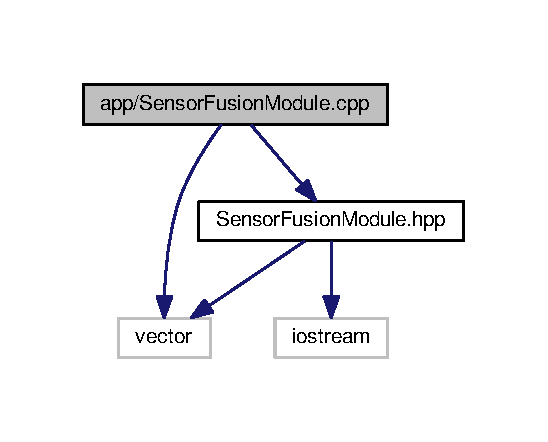
\includegraphics[width=263pt]{_sensor_fusion_module_8cpp__incl}
\end{center}
\end{figure}


\subsection{Detailed Description}
E\+N\+P\+M808X, Midsemester project. 

\begin{DoxyAuthor}{Author}
Karan Vivek Bhargava 
\end{DoxyAuthor}
\begin{DoxyCopyright}{Copyright}
M\+IT License
\end{DoxyCopyright}
\hypertarget{_robot_test_8cpp_DESCRIPTION}{}\subsection{D\+E\+S\+C\+R\+I\+P\+T\+I\+ON}\label{_robot_test_8cpp_DESCRIPTION}
This program is controlling a robot\textquotesingle{}s heading direction using sensor fusion. 